%!TEX root = ../paper.tex

\subsection{Web Browsing} \label{label:web}
\begin{figure}[t]
  \centering
  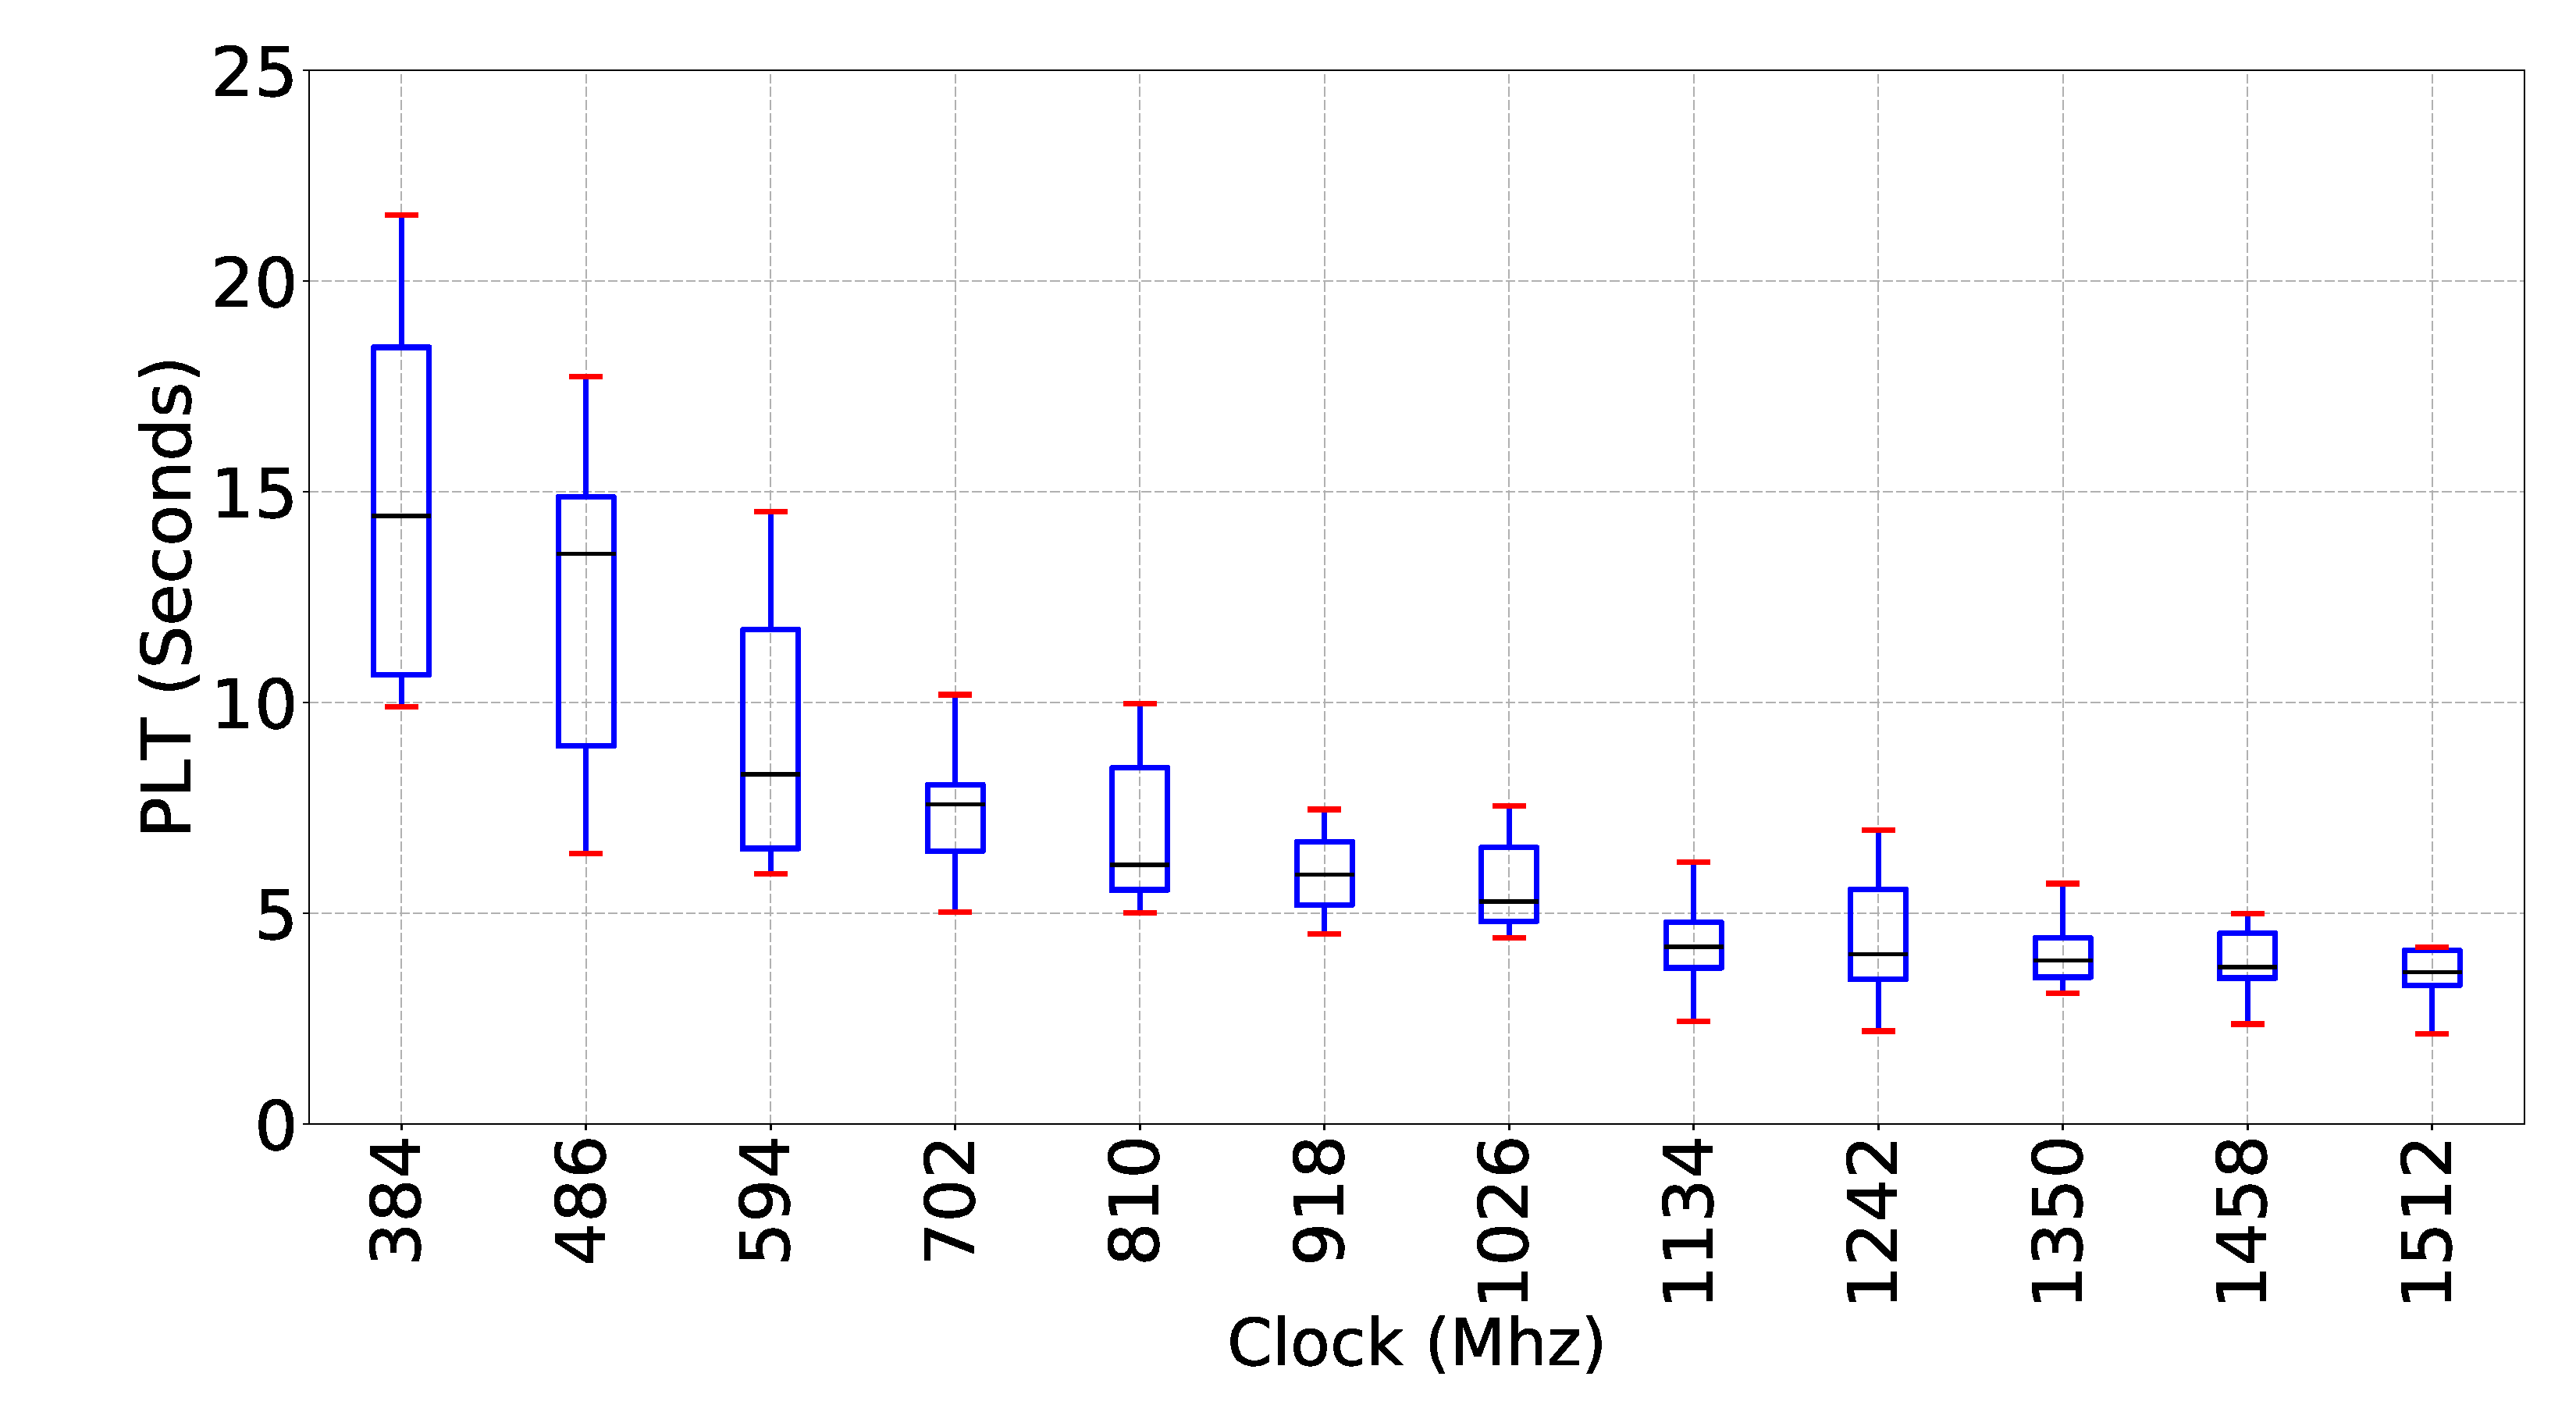
\includegraphics[width=0.9\linewidth]{sections/device-work/plt-clock}
    \caption{Web QoE: The average Page Load Time (PLT) across 12 different CPU speeds on Nexus 4. As the CPU speed decreases, PLT increases significantly. }
  \label{fig:plt_clock}
\end{figure}


Different from our earlier experiments (\S\ref{sec:motivation}) which were conducted across devices, in this section we study Web QoE  across 12 different CPU speeds on the same device. The experiments are repeated over three smartphones---Nexus 4, Intex Amaze+, and Google Pixel 2 (see Table~\ref{tab:device_types} for specs). The experiments involve loading the top 50 Websites from the Alexa suite~\cite{alexa}.  We use the 
same experimental set up as described in \S\ref{sec:setup}. The CPU speeds are changed using the governor~\cite{ad-governors}. We present the results from Nexus\,4 in detail and summarize the results from the other two phones for brevity.
%
Recall that the Web pages are hosted in a local server and accessed via a well-provisioned LAN so that the performance is not affected by the external network conditions. 

%Web browsing is more complex ecosystem than video applications because of its complex inter dependencies between network and compute activities. In this sectin, we first show the effect of clock on Web QoE and then explain the isolation of clock effect on network and compute. We load the top 50 Web pages from the Alexa list of top 50 Web sites and measure PLT using the setup described in \S\ref{sec:motivation}.

Figure \ref{fig:plt_clock} shows the average PLT across different CPU clock frequencies. The PLT increases 77\% when the CPU clock frequency drops from 1512\,MHz to 384\,MHz. The trends are similar to Figure~\ref{fig:motivation}a where the page loads much slower on low-end devices compared to higher-end devices. In other words, the performance of Web page loads on low-end devices is similar to that of a slower clock on a high-end device. 

\begin{figure}[t]
  \centering
  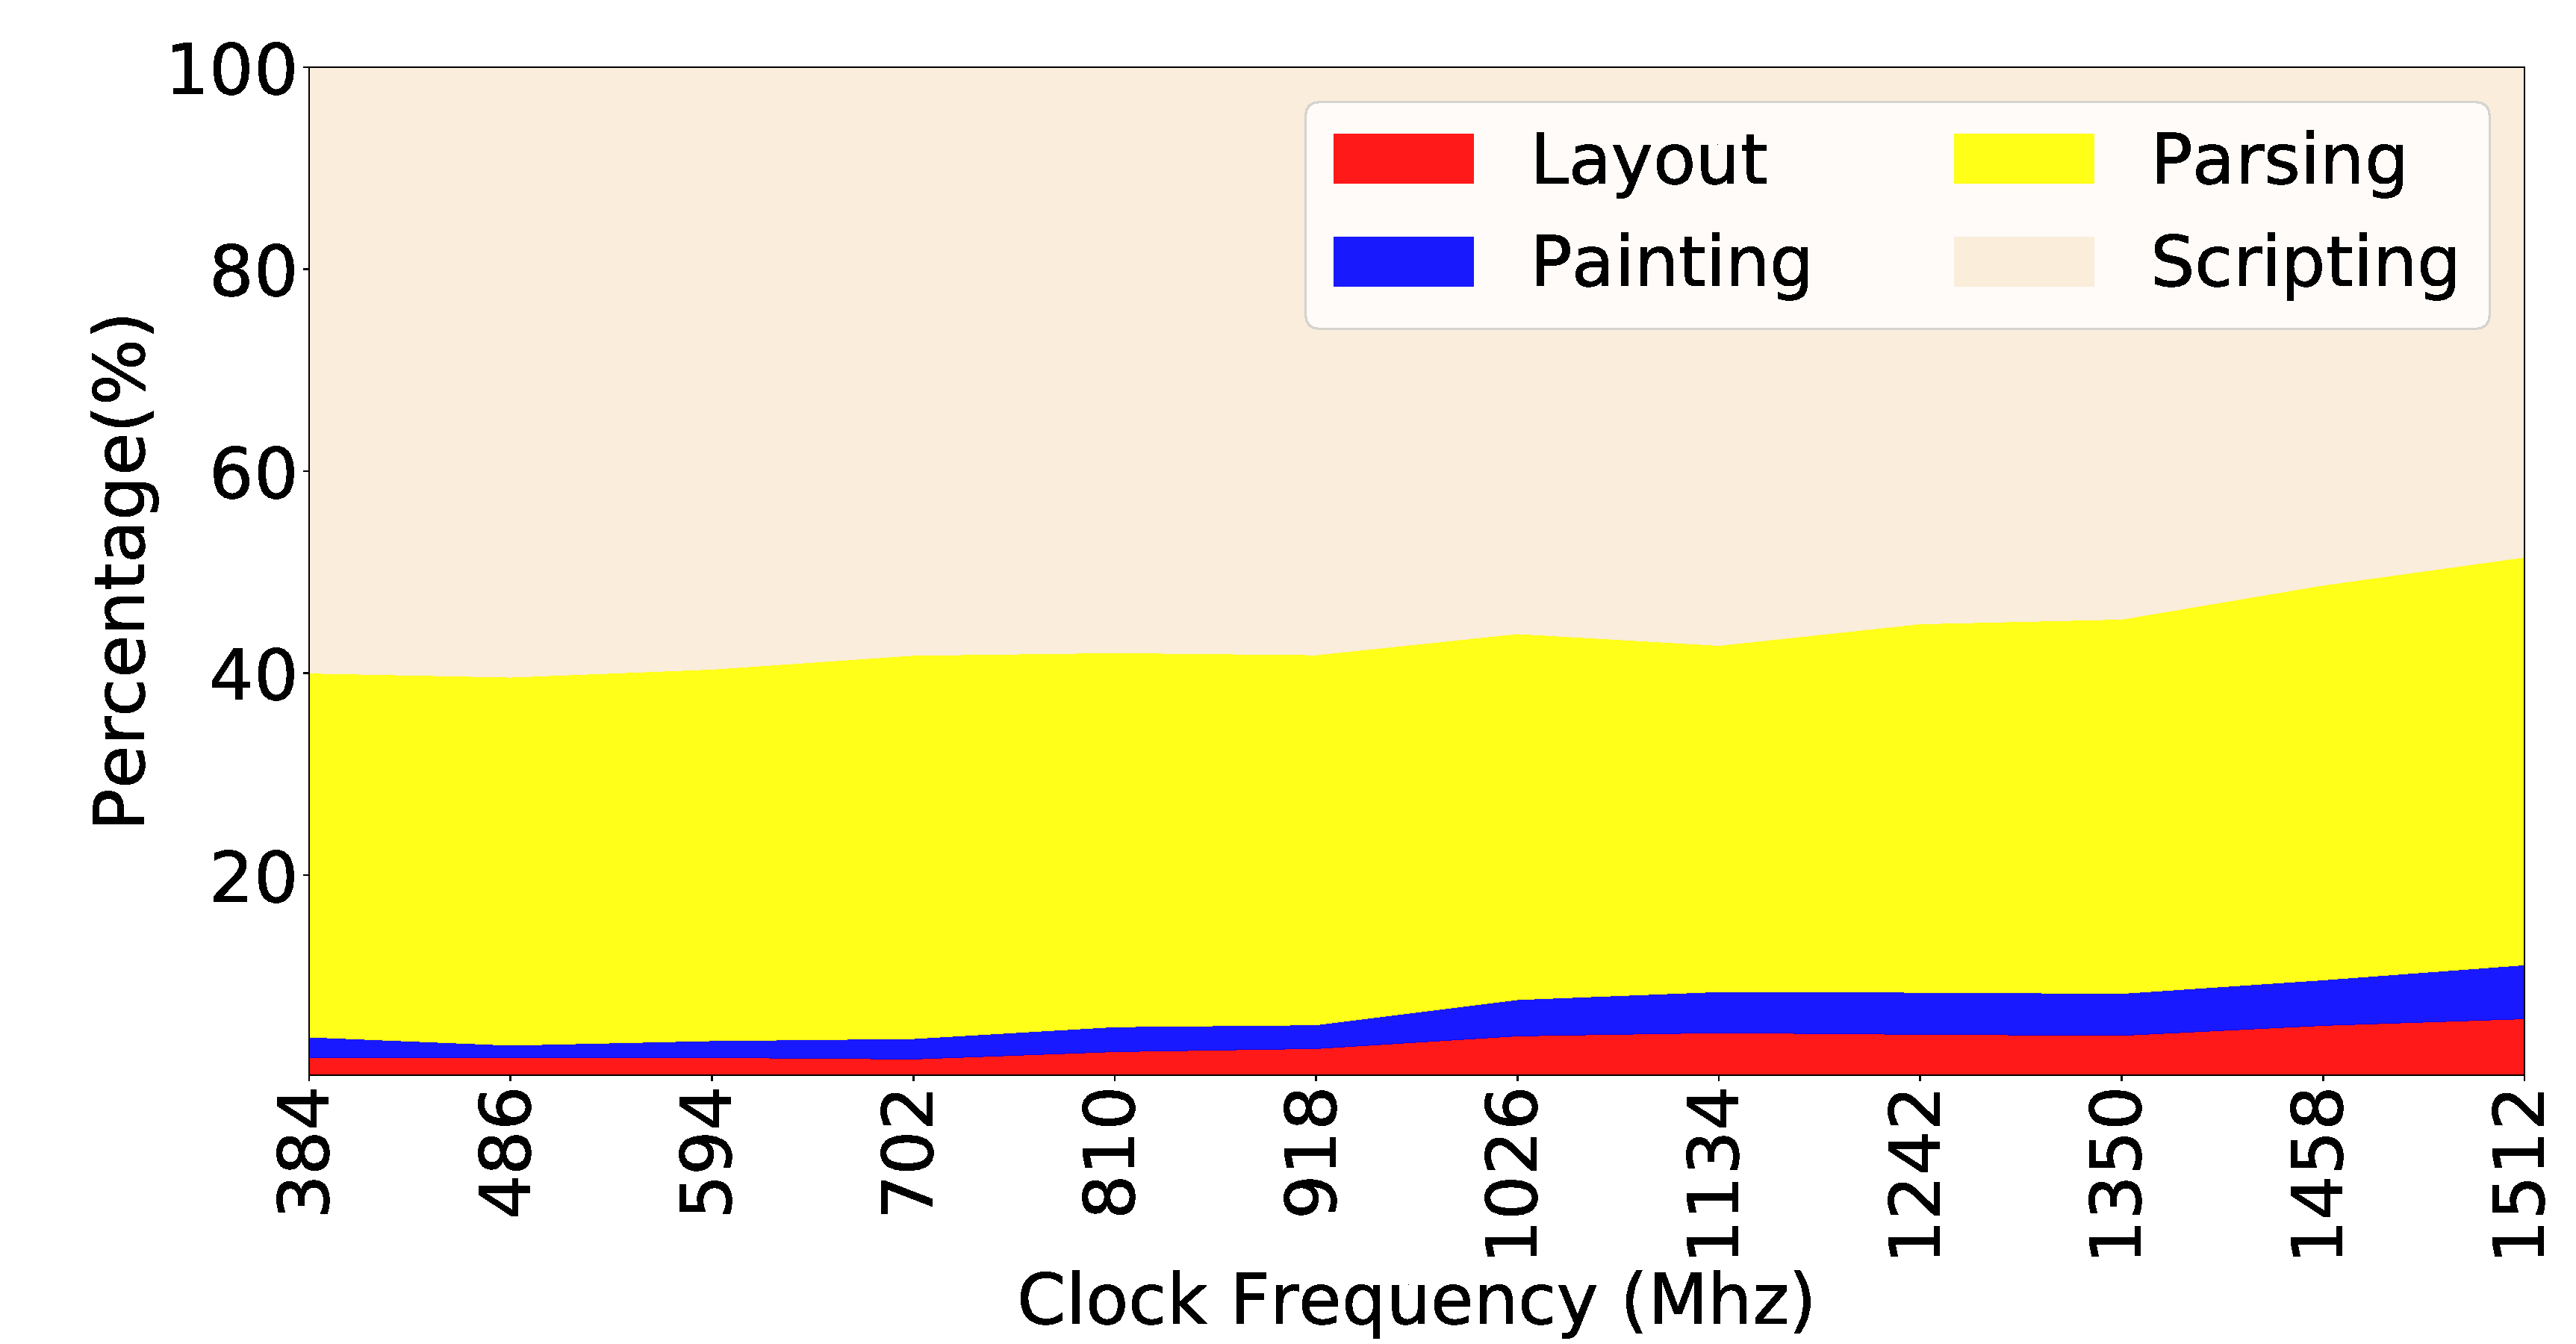
\includegraphics[width=\linewidth]{sections/device-work/plt-pie}
  \caption{The time spent on compute activities during page load is further divided into individual activities---Scripting (or Javascript evaluation), HTML Parsing, Layout, and Painting. The scripting time increases significantly when the CPU slows down.  }
  \label{fig:dissect}
\end{figure}
{\noindent \bf Impact of Network Vs. Compute:}
Our goal now is to determine if the poor Web QoE is because the network throughput drops under slow CPU speeds or  because of slower processing. Recall that the slow CPU speeds not only affects compute but also the network throughput due to the packet processing delays (\S\ref{label:throughput}). The problem is that during Web page loads, network and compute activities are interspersed, making it hard to cleanly separate the effect of network and compute. 

Instead, we leverage the WProf tool that extracts the timings of the network and compute activities of the page load process. Figure~\ref{fig:wprof-dp} shows the output provided by the WProf tool~\cite{wang2013demystifying,nejati2016depth} when loading an example page. In this example, the network components are shown in {\em green} and the compute components are shown in {\em blue}. WProf~\cite{wang2013demystifying} (and the version for mobile browsers, WProf-M~\cite{nejati2016depth}) first identifies the timing of each activity. WProf then extracts the dependencies between the activities and draws the dependency graph. For example, in Figure~\ref{fig:wprof-dp}, HTML parsing (6) cannot start until the Javascript (JS) is evaluated (5) because of dependencies between parsing and Javascript evaluation.  The critical path is the bottleneck path in the dependency graph (shown using the red line); the length of the critical path provides the PLT. %As the CPU speeds change, the dependency graph and the critical path change, making it hard to isolate the effect of network and compute.

Using WProf, we estimate the time on the critical path involving compute activities (HTML parsing, scripting, rendering, and CSS evaluation) and network activities (object loading) as shown in Figure~\ref{fig:plt_isolate}. The sum of the network and compute activities gives the PLT (the PLT numbers are from Figure~\ref{fig:plt_clock}). The network time on the critical path increases from an average of 2 seconds when the clock speed is 1512\,MHz to 6 seconds when the clock speed is increased to 384\,MHz -- a 66\% increase. The compute time increases by 76\% for the same CPU slow down. We find that the compute time increases even more compared to network time for more complex Webpages (not shown here). 

Figure~\ref{fig:dissect} further dissects the compute activities into HTML parsing, JS scripting, CSS evaluation, layout and painting. 
%We measure the fraction of time spent on these activities individually using WProf tool. 
Scripting times increase the most as the CPU clock slows down; it accounts for 51\% of the overall compute times at high CPU frequencies, and 60\% at low CPU frequencies. The layout and painting only account for 4\% of the compute time on the critical path. 

The  takeaway from Figure~\ref{fig:dissect} is that, a key component for improving Web page loads, especially at slow CPU speeds, is to  improve the efficiency of scripting. 
%
Figure~\ref{fig:sites-effect} demonstrates
this in another way -- Websites with a large number of Javascript are affected the most when the CPU slows down. In this experiment, we choose the top 50 pages from the  Alexa suite~\cite{alexa} under different categories -- kids and teen, health, shopping, news, and sports. 
%The categories are ordered according to the time spent on scripting/Javascript evaluation when the phone is operating at 1512\,MHz. 
The sports Webpages spend the most time on scripting and clearly suffers the maximum slow down (up to 13\,sec) when CPU frequency drops from the fastest
to the slowest. On the other hand, kids and teen Webpages increases by $<3.5$ seconds. We leverage this observation to improve Web page load performance (\S\ref{label:whatif}).

\begin{figure}[t]
  \centering
  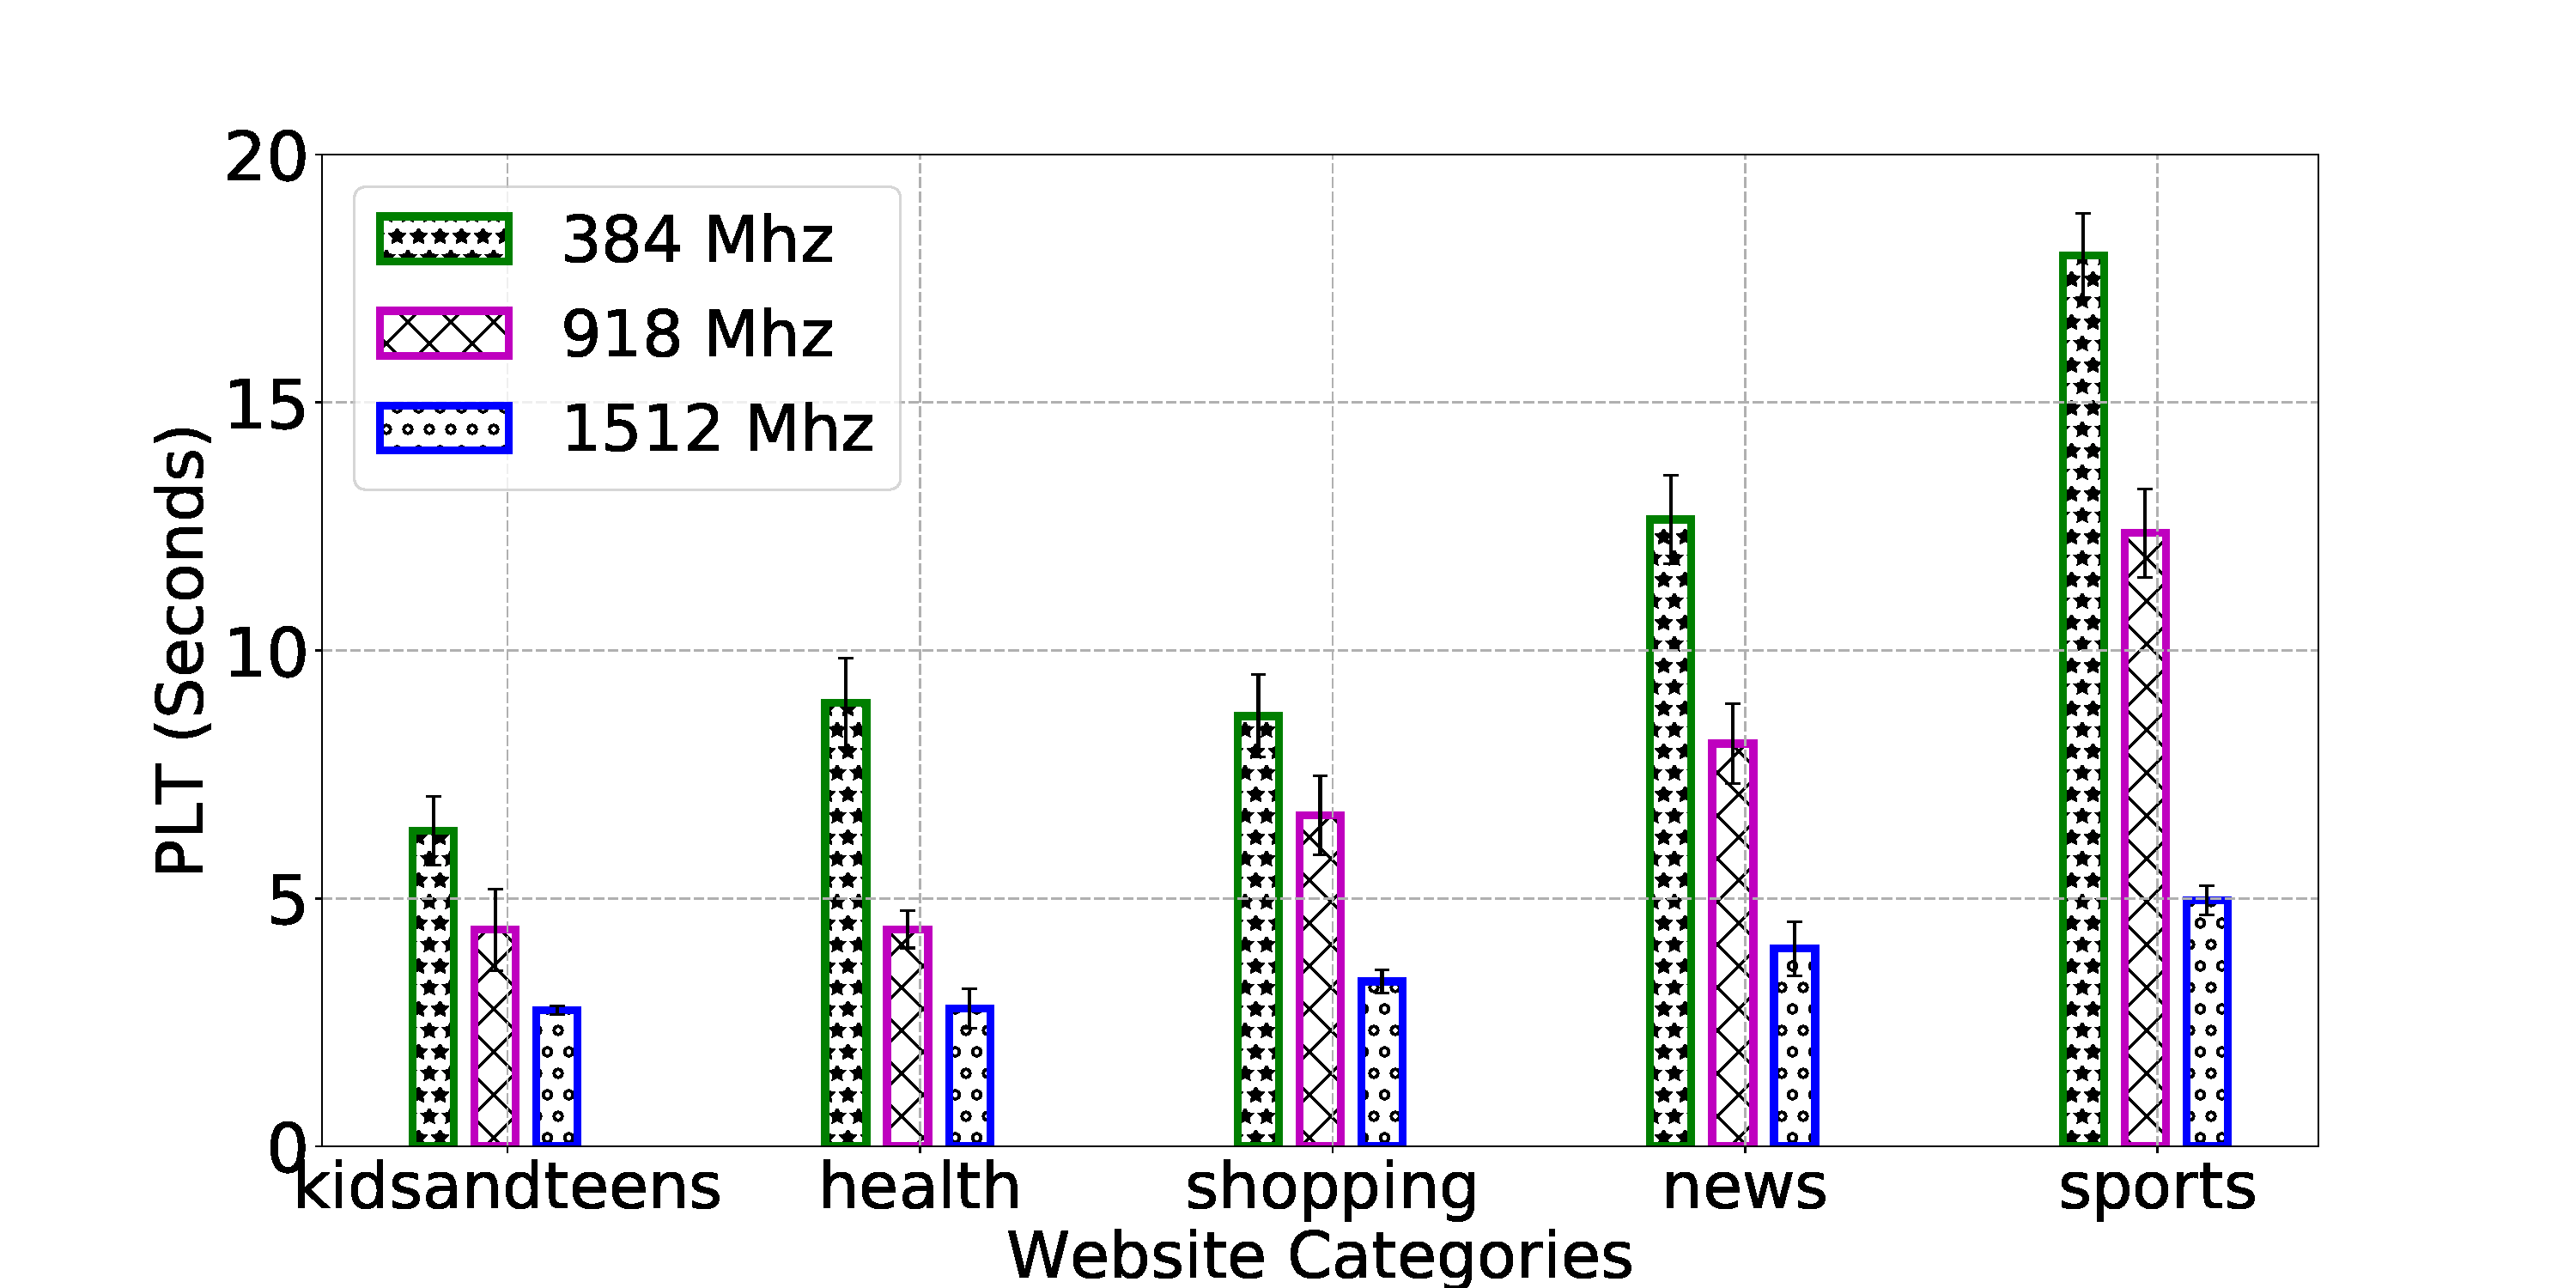
\includegraphics[width=\linewidth]{sections/device-work/sites-effect}
  \caption{PLT for three different CPU frequencies for different Webpage categories. The sports Webpages are Javascript-heavy and are affected the most by the CPU 
  slow down.    }
  \vspace{-0.2in}
  \label{fig:sites-effect}
\end{figure}

\begin{figure*}
    \begin{subfigure}[b]{0.5\textwidth}
        \centering
        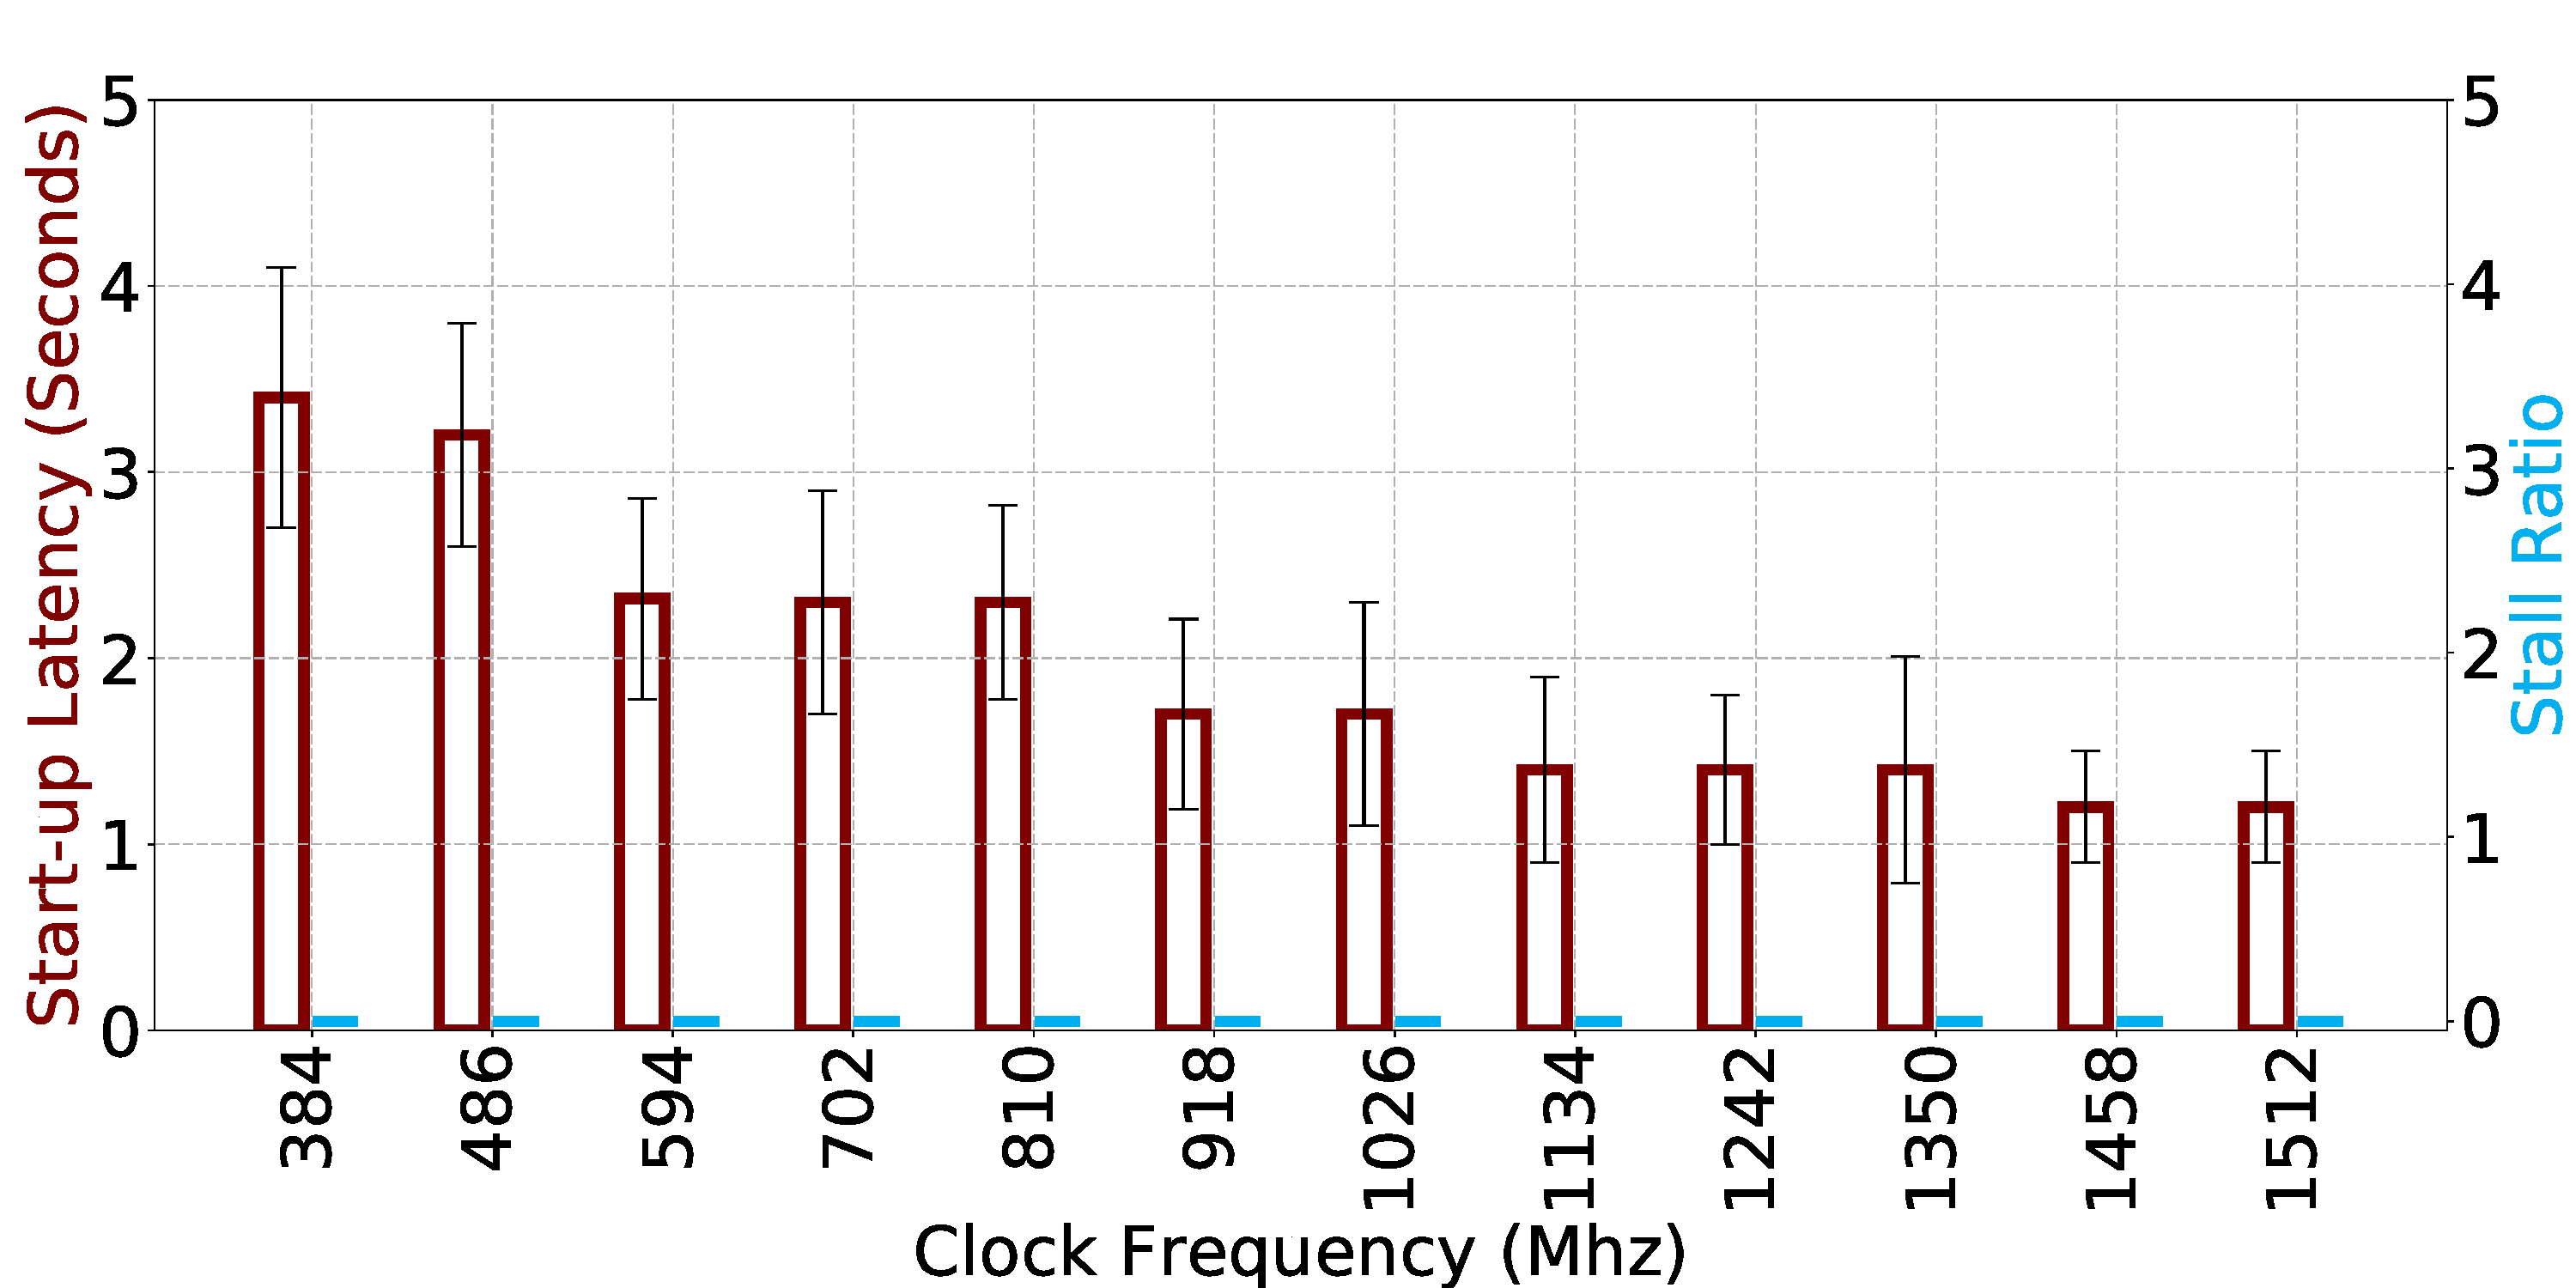
\includegraphics[height=0.5\textwidth,width=1\textwidth]{sections/device-work/youtube-clock}
        \caption{}
    \end{subfigure}
    \begin{subfigure}[b]{0.5\textwidth}
        \centering
        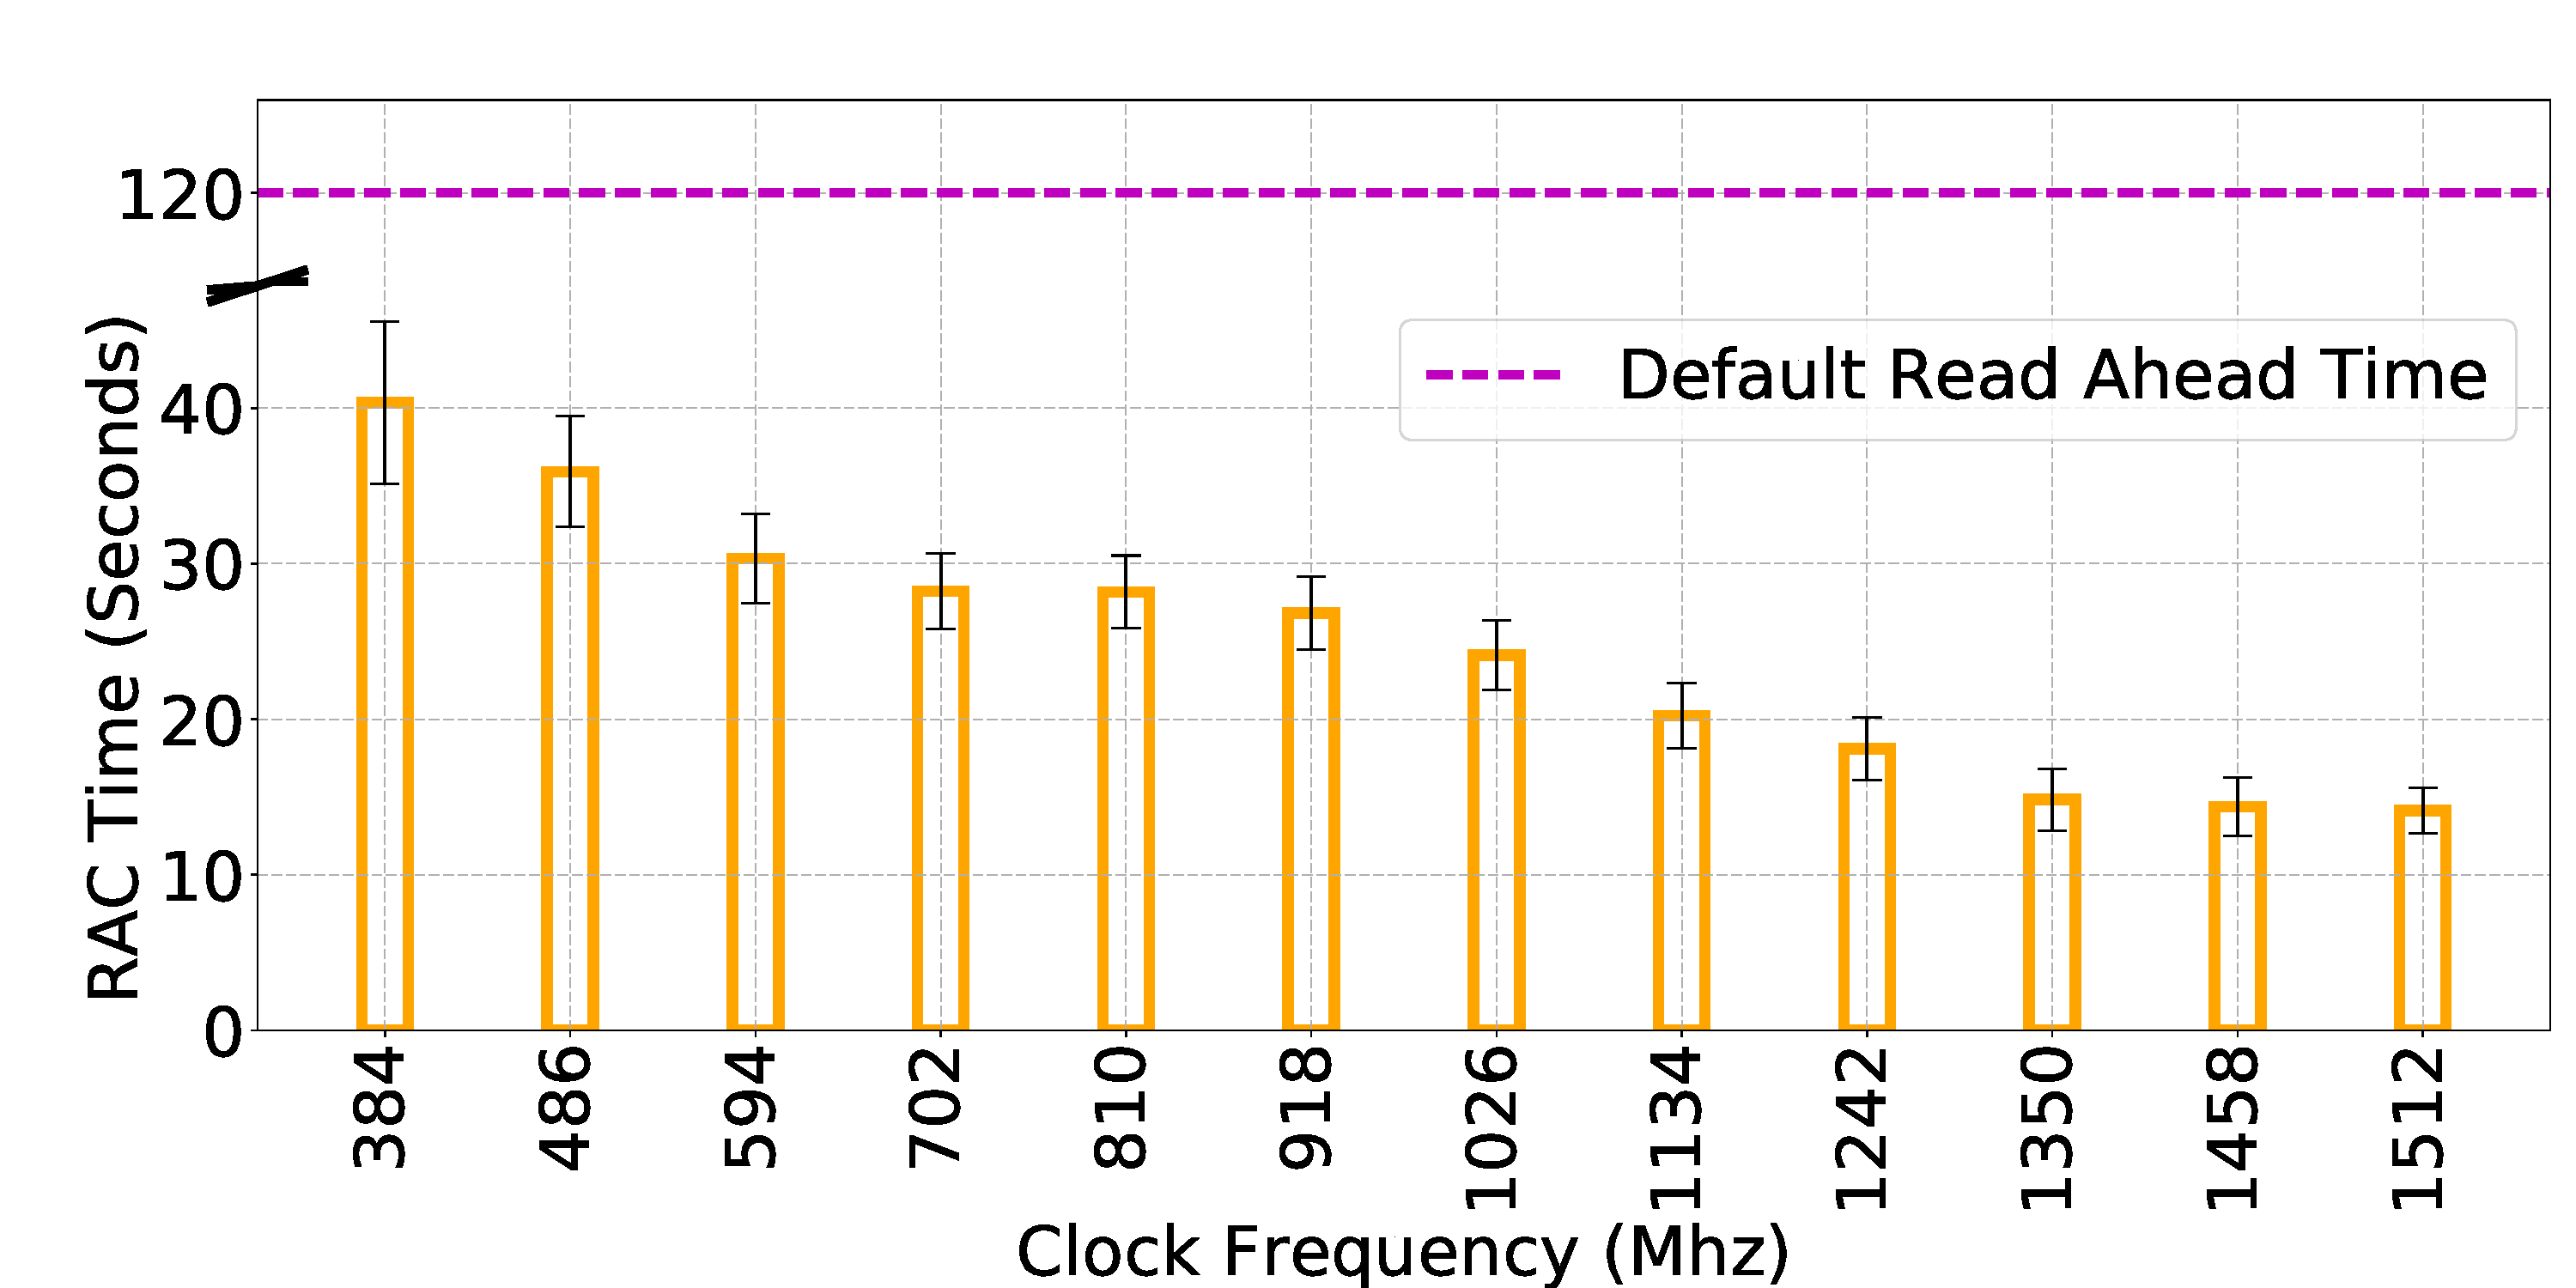
\includegraphics[height=0.5\textwidth,width=1\textwidth]{sections/device-work/youtube-rac}
        \caption{}
    \end{subfigure}%
    \caption{(a) Effect of CPU speeds on YouTube: The start-up latency is increased by 50\% but the stall ratio is not affected by the slow clock across the 12 CPU speeds. (b) Isolating the effect of network on stall ratio: The read-ahead convergence time (RAC) is the time required for YouTube to prefetch a read-ahead buffer worth of data (typically 120 seconds of video content). Even under slow clock, the time it takes to prefetch content is well below 120 seconds, which is the time it takes to play the content. As a result, read-ahead buffer is always full and the user does not experience stalls. }
   \vspace{-0.2in}
  \label{fig:youtube}
\end{figure*}
 

